\documentclass[margin,line]{res}
\usepackage{hyperref}
\usepackage{url}
\usepackage[export]{adjustbox}
\usepackage{graphicx}

\oddsidemargin -.5in
\evensidemargin -.5in
\textwidth=6.0in
\itemsep=0in
\parsep=0in
\topmargin=0in
\topskip=0in
 
\newenvironment{list1}{
  \begin{list}{\ding{113}}{%
      \setlength{\itemsep}{0in}
      \setlength{\parsep}{0in} \setlength{\parskip}{0in}
      \setlength{\topsep}{0in} \setlength{\partopsep}{0in}
      \setlength{\leftmargin}{0.17in}}}{\end{list}}
\newenvironment{list2}{
  \begin{list}{$\bullet$}{%
      \setlength{\itemsep}{0in}
      \setlength{\parsep}{0in} \setlength{\parskip}{0in}
      \setlength{\topsep}{0in} \setlength{\partopsep}{0in}
      \setlength{\leftmargin}{0.2in}}}{\end{list}}


    
\begin{document}
\hspace{5cm}
\name{\LARGE \hspace{7cm} Ashlesha Borade} 

\begin{resume}
\section{\bf ADDRESS:}

\begin{tabular}{@{}p{3.5in}p{3in}}
Government Girl's hostel             & {Contact:} +917038222736/9834803168 \\
Gov. College of Engg and Research 
 & {E-mail:}  ashlesha14061998@gmail.com\\
Avasari(Khurd), Tal. Ambegaon\\
Dist. Pune-412405\\
Maharashtra.
\end{tabular}

\begin{figure}[h]
	\hspace{11cm}
	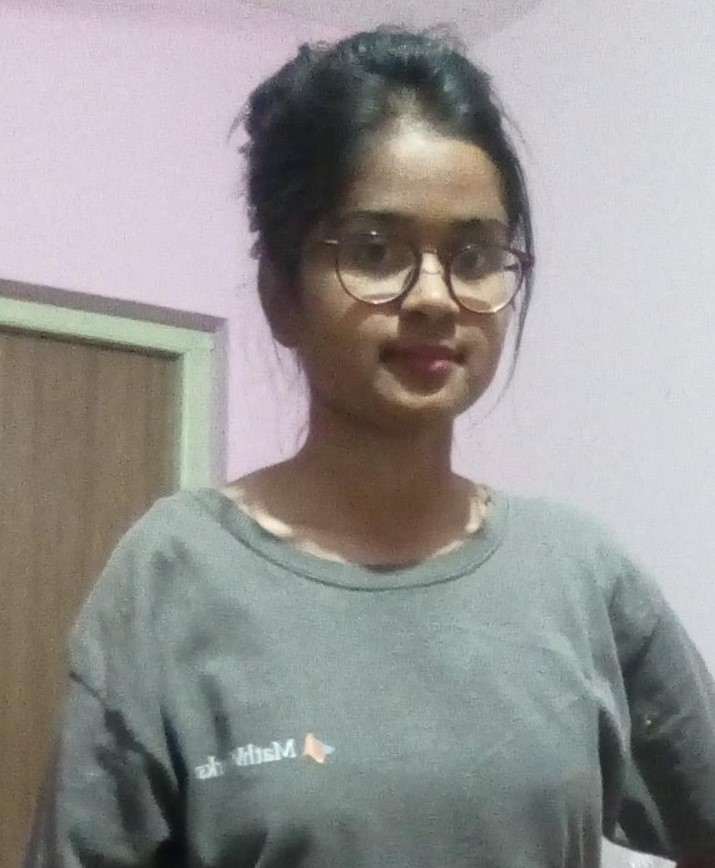
\includegraphics[width=0.2\textwidth]{E:/Ashlesha}
\end{figure}   

\section{\bf OBJECTIVE:}

To learn and contribute to the world's technical innovations and to improve the lifestyle of mankind through technology.

\section{\bf EDUCATION:}
\vspace{0.5cm}



\begin{tabular}{|p{1.5cm}|p{4.5cm}|p{3cm}|p{2.0cm}|p{1.7cm}|}
	\hline
	\textbf{Degree} & \textbf{College/ School} & \textbf{University} & \textbf{Passing Year} & \textbf{Pass Percentage}\\ [0.5ex] 
	\hline
	3rd Year B.E . &Govt. College of Engineering \& Research avasari(khurd)   &SPPU &Pursuing& - \\ 
	\hline
	2nd Year B.E. &Govt. College of Engineering \& Research avasari(khurd) &SPPU &2017-18& 8.36 SGPA \\ 
	\hline
	HSC & Sona "I" Englsh Medium School and Jr. college& Pune University  &2015-16 & 81.54 \\
	\hline
	SSC &Sona "I" Englsh Medium School and Jr. college) &Pune University&2013-14&93.60\\
        \hline
\end{tabular}

\hfill 

\section{\bf{\Large{Projects:}}}
\begin{enumerate}
	\item{{\textbf{\large{Rongbay:}}}\\ 
		The theme of ABU Robocon 2018 in which we built manual \& automatic robot , throwing 					mehanism,etc.}


	\item{{\textbf{\large{Nutty Squirrel:}}}\\ The theme of eYantra Robotics Competition organised \& held at IIT Bombay based on electronics \& computer engineering technical aspects \& were the finalist \& also received the "Consolation Prize" for the same }


\end{enumerate}
\hfill



{\section{\Large\bf{Training and internship:}}}
\begin{enumerate}
\vspace{1cm}
	\item{BSNL Training course on "Broadband Technician" at Regional Telecommunication Training Centre, Pimpri Chichwad. }	

	\item{ Workshops attended on Raspberry pi, Andriod App Development at COEP, Matlab \& Simulink 			at MITCOE. }	
\end{enumerate}
\hfill

{\section{\Large\bf{Research Publications:}}}
\begin{itemize}
	\item{Yet to do.}	
\end{itemize}
\hfill






{\section{\Large\bf{Technical skills}}}
\begin{enumerate}
	\item{Programming in C, C++ ,embedded C, basics of JAVA and python.}
	\item{Microsoft Office(Word, Excel, Powerpoint).}
	\item{Matlab \& Simulnk, Scilab.}
	\item{HTML, Latex, LINUX commands.}
	\item{Workded on various softwares like Atmel Studio 7 , keil uVision , Proteus,arduino IDE , IntelliJ IDEA, Matlab and Simulink, Adobe Photoshop , andriod studio, V-REP , Visual Studio  etc.}
\end{enumerate}
\hfill






{\section{\Large\bf{Soft Skills:}}}
\begin{enumerate}
	\item{Confident \& Good Speaker.}
	\item{Consistency.}
	\item{Positive attitude and Successful management in various activities in school, colleges.}	
	\item{Better Communication skills.}
	\item{Creative in Art and drawings.}	
\end{enumerate}
\hfill





{\section{\Large\bf{Extra Curricular Activities:}}}
\begin{enumerate}
	\item{Participation in "eYantra Robotics Competiton (eYRC)" \& received the "Consolation Prize" for the same 			conducted at IIT Bombay .}
	\item{Participation in ABU ROBOCON INTERNATIONAL EVENT 2018 : “RONGBAY” \& received the "Smart 				Robot " Award from ROBOU.}
	\item{Member of ROBOTICS RESEARCH LAB (1 yr. experience).}
	\item{Senior member of eLSI Laboratoary \& run various activites for juniors in the college} 

	\end{enumerate}
\hfill





{\section{\Large\bf{Co-Curricular Activities:}}}
\begin{enumerate}
	\item{Co-ordinator of "ROBOx competition"  in ABINITO 2018-19 National Technical Event..}
	\item{Volunteer of "CIRCUITRIX competition" in ABINIITO 2017-18 National Technical Event.}
	 \item{"Cultural Secretary" of Department in the college.}
	 \item{Volunteer of "Electronics and Telecommunication Student Association (ETSA)" in the college.}
	 \item{"Volunteer of Training and Placement Office (TPO) of college and run various activities under college.}
	 \item{Actively participating every year in various Indoor Competitions like Carrom, Chess, etc .}
	

\end{enumerate}
\hfill






{\section{\Large\bf{Personal details:}}}
\begin{itemize}
	\item{Father's name: Maruti Gulabrao Borade}
	\item{Mother's name: Sandhya Maruti Borade}
	\item{Sex: Female} 
	\item{Nationality: Indian} 
	\item{Languages known: English, Hindi, Marathi, Gujarati} 
	\item{Date of Birth: 14/06/1998} 
\end{itemize}
\hfill






{\section{\Large \bf{Reference:}}} 
Dr. Niteen P. Futane\\
Professor\\
Government College of Engineering And Research Avasari(khurd)\\
ph number- +91 9004828465\\
email- niteen\_futane10@redifmail.com\\
\hfill\\

{\section{\Large \bf{Declaration:}}} 

	I do hereby assure that the above information is truthful to the best of my cognition.
\hfill\\

{\section{\Large \bf{Date:}}}  14/4/2019



\end{resume}
\end{document}




